\FloatBarrier
\begin{figure}[!h]
\begin{subfigure}[t]{0.5\textwidth}
	\centering
	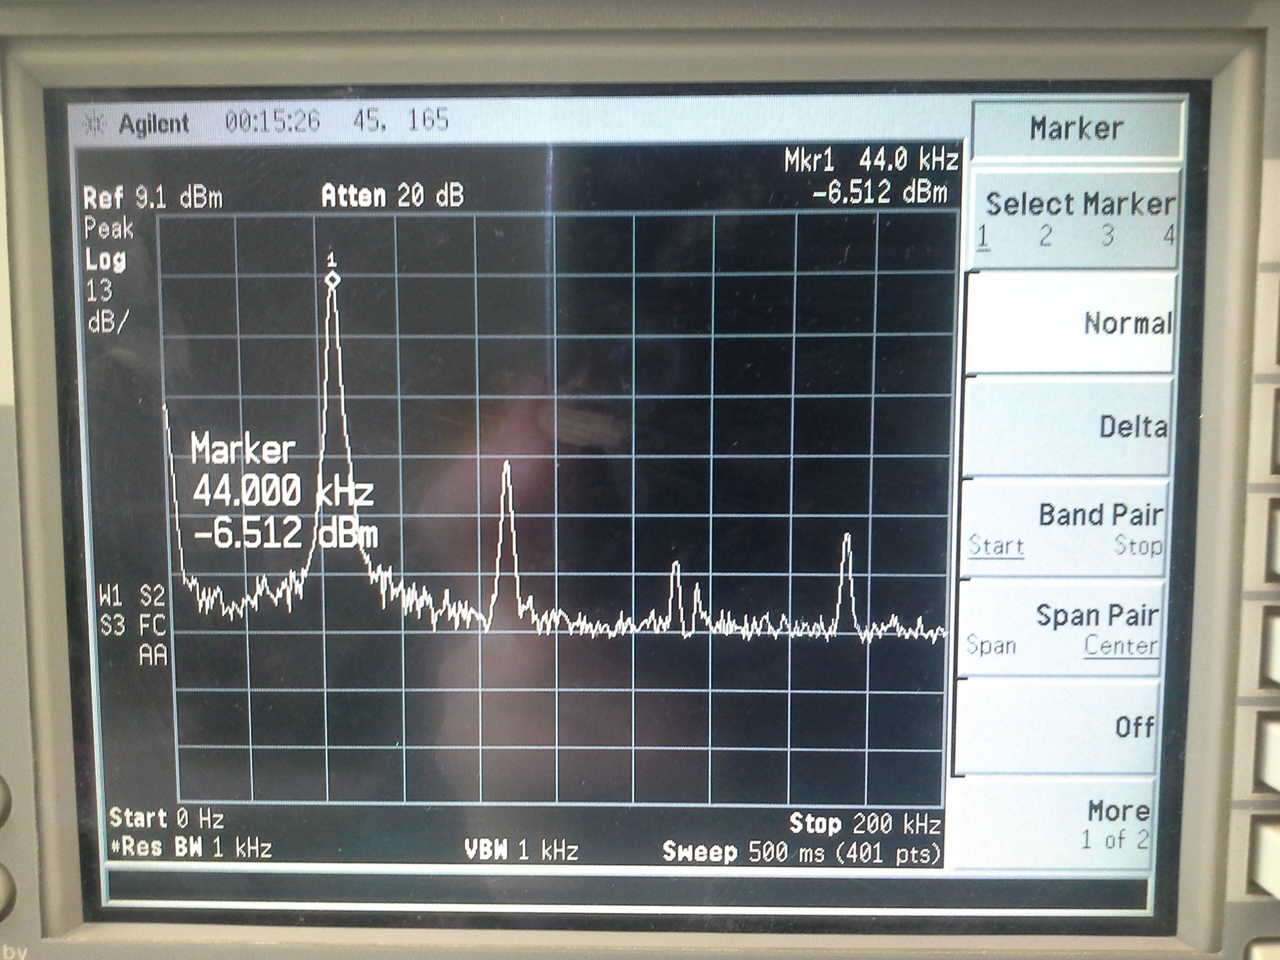
\includegraphics[scale=0.17]{../Grafiken/ModulationsspannungOberwellen_0.jpg}
	\caption{Grundschwingung \label{fig:modulationsspannungoberwellen_0}}
\end{subfigure}%
~
\begin{subfigure}[t]{0.5\textwidth}
	\centering
	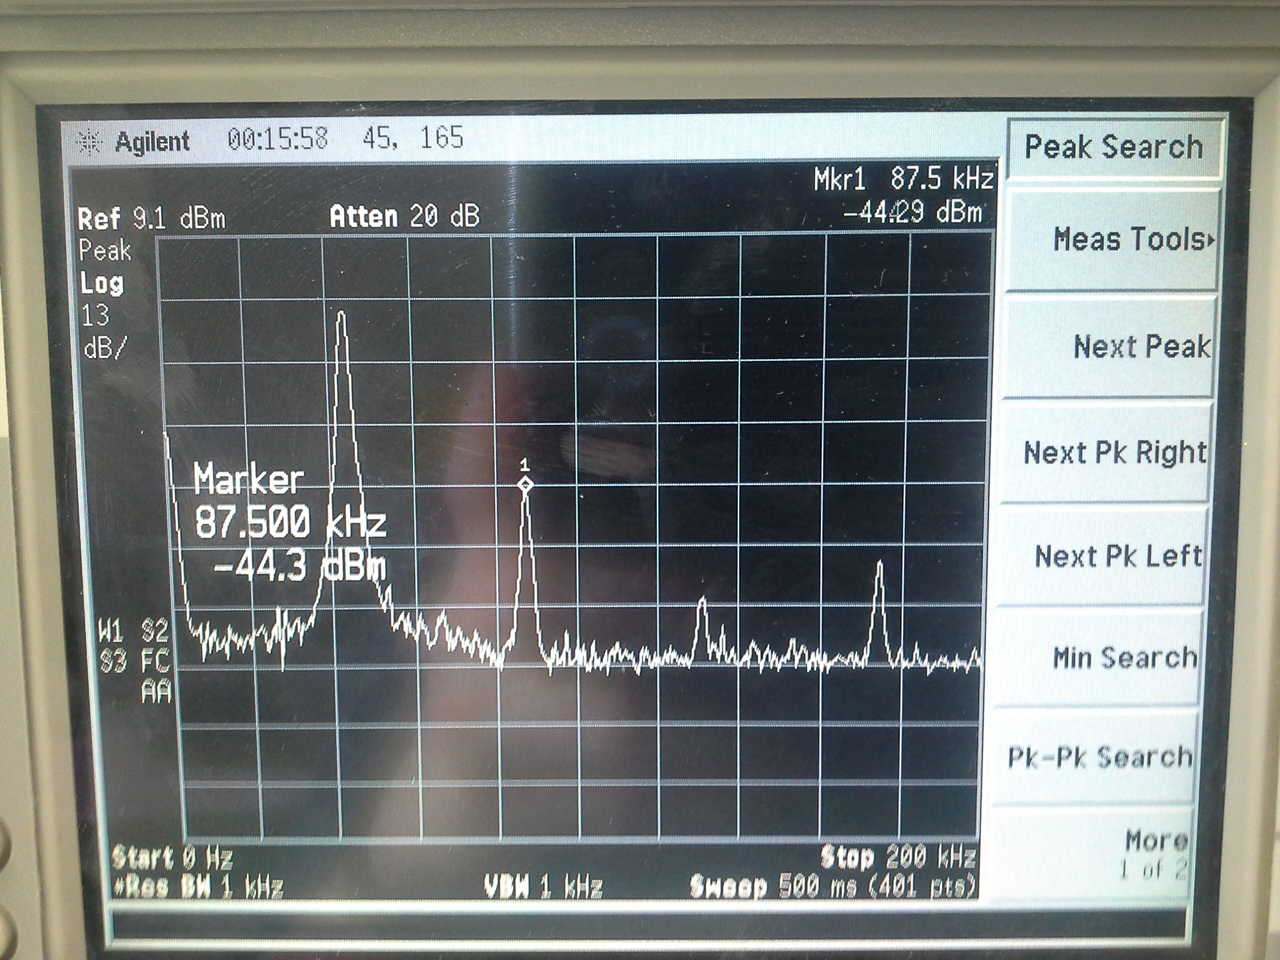
\includegraphics[scale=0.17]{../Grafiken/ModulationsspannungOberwellen_1.jpg}
	\caption{Erste Oberschwingung\label{fig:modulationsspannungoberwellen_1}}
\end{subfigure}
	\caption{Frequenzspektrum der verwendeten Modulationsspannung. Zu erkennen sind die Oberschwingungen,
		     die bereits in der ursprünglichen Spannung vorhanden sind. \label{fig:modulationsspannungoberwellen}}
\end{figure}
\FloatBarrier